\chapter{Introduction}

\section{The standard model of particle physics}

The success of modern particle physics, since its inception in 1970s, 
is summarized as the Standard Model (SM) of particle physics.
It is a formulation that describes all known elementary particles, 
and three of the four known fundamental interactions between them:
the electromagnetic, weak, and strong interactions, but not the gravitational interaction whose quantization is not yet confirmed.
Elementary particles can be classified into fermions and bosons, based on their spins.
Elementary fermions are spin 1/2 particles that form matter in the macroscopic world as we know,
while elementary bosons have integer spins (0 or 1) and are the carrier of particle interactions.
Fermions are further categorized into quarks and leptons, each has three generations.
In each generation, there is one charge = $+\frac{2}{3}$ quark (u, c, and \Pqt for each generation), 
one charge = $-\frac{1}{3}$ quark (d, s, and \Pqb), one charge = 1 lepton ($\Pe$, \mu, and \tau), 
and one neutral lepton ($\nu_{e}$, $\nu_{\mu}$, and $\nu_{\tau}$). 
Each of these particles is complemented with an anti-particle which has the same mass and spin as the particle itself, 
but opposite charge and other quantum numbers.
There are two types of elementary bosons, the vector bosons (also called gauge bosons) that have spin = 1 and the scalar boson with has spin = 0.
Gauge bosons are the carriers of fundamental interactions: photons for the electromagnetic interaction, the \PW and \PZ bosons for the weak interaction,
and gluons for the strong interaction.
The Higgs boson is the only scalar boson in the SM, 
which couples to all massive elementary particles and provide the mechanism for them to be massive.
The elementary particles of the SM is summarized in Figure~\ref{fig:SM_table}.

\begin{figure*}[!htb]
    \centering
    \captionsetup{justification=justified}
    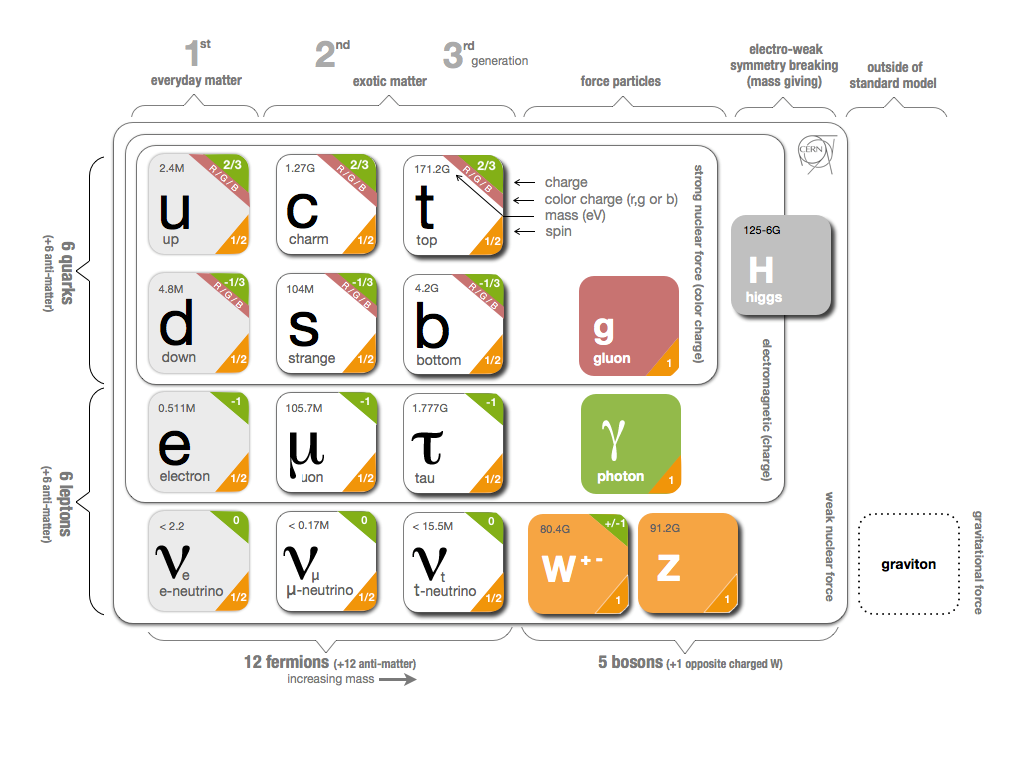
\includegraphics[width=0.9\textwidth]{pics/Intro/standard_model_cern.png}
    \caption{The Standard Model of particles physics: 12 elementary fermions and 5 elementary bosons.
             Photo taken from~\cite{SM_table_CERN}. }
    \label{fig:SM_table}
\end{figure*}

The SM is mathematically constructed within Quantum Field Theory with a structure of the product of an SU(3), an SU(2), and an U(1) groups.
The Lagrangian density of the SM is expressed as:
\begin{equation}\label{eq:SM_Lagrangian}
  \begin{split}
    \mathcal{L} = & \bar{\psi}^{i} (i\gamma^{\mu})(\mathcal{D}_{\mu})_{ij}\psi^{j} -
                  - \frac{1}{4} G^{a}_{\mu\nu}G^{a\mu\nu}
                  - \frac{1}{4} W^{a}_{\mu\nu}W^{a\mu\nu}
                  - \frac{1}{4} B_{\mu\nu}B^{\mu\nu} \\
                & - m_{f} \bar{\psi}^{i}_{f} \psi_{fi}
                  + \frac{1}{2} m^{2}_{G} G_{\mu}G^{\mu}
                  + \frac{1}{2} m^{2}_{W} W_{\mu}W^{\mu}
                  + \frac{1}{2} m^{2}_{B} B_{\mu}B^{\mu}
  \end{split}
\end{equation}
In the equation:
\begin{itemize}
  \item $\psi$ is the fermion field (matter field);
  \item $G^{a}_{\mu\nu}$, $W^{a}_{\mu\nu}$, and $B_{\mu\nu}$ are field strength tensors for the interaction fields 
        corresponding to the groups SU(3), an SU(2), and an U(1), respectively;
  \item $\mathcal{D}_{\mu}$ is the covariant derivative operator: $\mathcal{D}_{\mu}\psi = (\partial_{\mu} - ig^{\prime}B_{\mu}Y - igW^{a}_{\mu}T^{a} - ig_{s}G^{a}_{\mu}t^{a})\psi$,
        $g^{\prime}$, $g$, and $g_{s}$ being field strength coefficients, and $Y$, $T^{a}$, and $t^{a}$ being interaction operators;
  \item Index $a$ is the index of the group generators, which runs from 1 to 8 for the gluon, and 1 to 3 for the \PW boson;
  \item $m_{f}$, $m_{G}$, $m_{W}$, and $m_{B}$ are the masses of the fermion, gluon, \PW boson, and the neutral gauge boson;
  \item $\mu$ and $\nu$ are the Lorentz vector indices.
\end{itemize}

The second line in Equation~\ref{eq:SM_Lagrangian} indicates that fermions and gauge bosons can be massive.
However, these terms unlike the terms in the first line, are not invariant under local gauge transformation.
An additional scalar field is introduced, which interacts with the fermion and boson fields,
leading to a spontaneous symmetry breaking and allowing the mass terms to appear in Equation~\ref{eq:SM_Lagrangian} without violating gauge invariance.
This is scalar field is called the Higgs field and its effect is called the Higgs mechanism.

% Higgs self
The Higgs field is a complex scalar field whose potential is:
\begin{equation} \label{eq:Higgs_potential}
    V(\Phi) = - \mu^{2} \Phi^{\dagger}\Phi + \lambda(\Phi^{\dagger}\Phi)^{2}
\end{equation}
in which $\Phi$ is the complex scalar field and $\mu$, $\lambda$ are coefficients.
$\lambda$ needs to be positive for $V(\Phi)$ to have a minimum value.
If $\mu^{2} = 0$, the minimum of $V(\Phi)$ is zero, when $|\Phi| = 0$,
and the no mass is raised for the fermions and bosons.
If $\mu^{2} < 0$, $V(\Phi)$ shall have a nonzero minimum value when $|\Phi^{\dagger}\Phi| = \frac{\mu^{2}}{2\lambda}$.
In gauge transformation, when reducing $\Phi$ to a real scalar field $\phi$,
it can be rewrote as $\phi = \nu + h$, where $\nu = \frac{\mu^{2}}{\lambda}$ is a constant,
the Lagrangian of the Higgs field can be written as:
\begin{equation}\label{eq:Higgs_Lagrangian}
    \mathcal{L}_{H} = - V(\Phi) = -\lambda \nu^{2} h^{2} - \lambda \nu h^{3} - \frac{\lambda}{4} h^{4} + const.
\end{equation}
in which the first term is the mass term of the Higgs boson, the second term is the tri-Higgs coupling vertex term,
and the third term is the quad-Higgs coupling term.
The Higgs mass, from the first term, is:
\begin{equation}\label{eq:Higgs_mass}
    m_{h} = \sqrt{2 \lambda} \nu   
\end{equation}
where $\nu$ can be determined from theory $\nu = $ 246 \GeV, while $\lambda$ is an unknown parameter.

% Higgs gauge
Adding the Higgs field to a massless SM Lagrangian, the Lagrangian becomes:
\begin{equation}\label{eq:SM_Lagrangian_Higgs}
  \begin{split}
    \mathcal{L} = & \bar{\psi}^{i} (i\gamma^{\mu})(\mathcal{D}_{\mu})_{ij}\psi^{j} -
                  - \frac{1}{4} G^{a}_{\mu\nu}G^{a\mu\nu}
                  - \frac{1}{4} W^{a}_{\mu\nu}W^{a\mu\nu}
                  - \frac{1}{4} B_{\mu\nu}B^{\mu\nu} \\
                & + \mu^{2} \Phi^{\dagger}\Phi - \lambda (\Phi^{\dagger}\Phi)^{2} \\
                & + (\mathcal{D}_{\mu}\Phi)^{\dagger} (\mathcal{D}^{\mu}\Phi)  \\
                & - y_{e} \bar{L}^{L} \Phi{} e_{R}
                  - y_{u} \bar{Q}_{L} \bar{\Phi} u_{R}
                  - y_{d} \bar{Q}_{L} \Phi{} d_{R} + \text(h.c.)
  \end{split} 
\end{equation}
where the first line is the massless SM terms, the second line is the Higgs self-interaction term,
the third line is the Higgs-gauge interaction term, and the fourth line is the Higgs-fermion interaction term.

The Higgs-gauge term can be expanded as:
\begin{equation}\label{eq:Higgs_gauge}
  \begin{split}
    (\mathcal{D}_{\mu}\Phi)^{\dagger} (\mathcal{D}^{\mu}\Phi) = &   \frac{1}{2} (\partial_{\mu} h)(\partial^{\mu} h) \\
                                                                & + \frac{g^{2}\nu^{2}}{4} W^{+}_{\mu} W^{-}_{\mu}
                                                                  + \frac{(g^{2}+{g^{\prime}}^{2}) \nu^{2}}{8} Z_{\mu} Z^{\mu} \\
                                                                & + \frac{g^{2}\nu}{2} h W^{+}_{\mu} W^{-}_{\mu}
                                                                  + \frac{g^{2}}{2} hh W^{+}_{\mu} W^{-}_{\mu} \\
                                                                & + \frac{(g^{2}+{g^{\prime}}^{2}) \nu}{4} h Z_{\mu} Z^{\mu}
                                                                  + \frac{g^{2}+{g^{\prime}}^{2}}{8} hh Z_{\mu} Z^{\mu}
  \end{split}
\end{equation} 
in which the first line is the Higgs kinetic term, the second line is the mass terms for \PW and \PZ bosons,
the third line is the hWW and hhWW interaction vertices, and the fourth line is the hZZ and hhZZ interaction vertices.
From this Lagrangian, the \PW and \PZ boson have masses of 
\begin{equation}\label{eq:gauge_mass}
  \begin{split}
    m_{W} & = \frac{g\nu}{2} \\
    m_{Z} & = \frac{\nu}{2} \sqrt{g^{2}+{g^{\prime}}^{2}}
  \end{split}
\end{equation}

%Higgs Yukawa
The Higgs-fermion terms, also called the Yukawa term, can be expanded as:
\begin{equation}\label{eq:Higgs_Yukawa}
  \begin{split}
    \mathcal{L}_{Yukawa} = & - (\frac{y_{e}\nu}{\sqrt{2}}) \bar{e}e - \frac{y_{e}}{\sqrt{2}} h \bar{e}e \\
                           & - (\frac{y_{u}\nu}{\sqrt{2}}) \bar{u}u - \frac{y_{u}}{\sqrt{2}} h \bar{u}u \\
                           & - (\frac{y_{d}\nu}{\sqrt{2}}) \bar{d}d - \frac{y_{d}}{\sqrt{2}} h \bar{d}d \\
  \end{split}
\end{equation}
in which the each line has a fermion mass term and a Higgs-fermion vertex term,
and the three lines are for leptons, up-type quarks, and down-type quarks, respectively.
As a result, the masses of leptons and two types of quarks are
\begin{equation}\label{eq:fermion_mass}
    m_{e} = \frac{y_{e}\nu}{2}, ~~~~~~~  m_{u} = \frac{y_{u}\nu}{2}, ~~~~~~~  m_{d} = \frac{y_{d}\nu}{2}
\end{equation}

Overall, fermions, the \PW, \PZ bosons, and the Higgs boson itself are allowed to be massive through the Higgs mechanism (Equations~\ref{eq:Higgs_mass}, \ref{eq:gauge_mass}, and \ref{eq:fermion_mass}).
The Higgs mechanism is experimentally confirmed by the observation of the Higgs boson by ATLAS and CMS Collaborations in 2012~\cite{Aad:2012tfa, Chatrchyan:2012xdj, Chatrchyan:2013lba},
while the latest and most precise measurement of the Higgs mass is $125.38 \pm 0.14$ \GeV from the CMS Collaboration~\cite{2020135425}.  
Furthermore, the Higgs boson couples to the \PW, \PZ bosons through gauge coupling, whose coupling strength is proportional to the mass of the gauge boson.
Similarly, the Higgs boson couples to fermions through Yukawa coupling, whose coupling strength is also proportional to the mass of the fermion.
Therefore, precise measurements of the Higgs coupling strength to different particles are keys to further validate the SM and search for new physics beyond the SM.


\section{The measurements of Higgs couplings}

The Higgs boson couples to all massive elementary particles, and can decay to most of them (except the top quark whose mass is greater than the Higgs boson).
The branching fractions of the decays are directly related to the coupling strength.
The Higgs boson can also decay to massless particles (gluons and photons) through top-quark-induced or \PW-boson-induced loop diagrams.
Table~\ref{tab:higgs_BR} lists the branching fractions of the main decay modes of the Higgs boson.

\begin{table}[!htb]
  \centering
  \captionsetup{justification=justified}
  \topcaption{The branching fractions of the main decay modes of the SM Higgs boson with a mass of 125 \GeV.}
  \begin{tabular}{lc}
    \hline
    Decay mode                 &  Branching fraction \\
    \hline
    $\PH \to \Pqb\Paqb$        &  58.4\% \\
    $\PH \to \PW^{+}\PW^{-}$   &  21.4\% \\
    $\PH \to gg$               &  8.19\% \\
    $\PH \to \tau\bar{\tau}$   &  6.26\% \\
    $\PH \to c\bar{c}$         &  2.89\% \\
    $\PH \to \PZ\PZ$           &  2.62\% \\
    $\PH \to \gamma\gamma$     &  0.227\% \\
    $\PH \to \PZ\gamma$        &  0.153\% \\
    $\PH \to \mu\bar{\mu}$     &  0.022\% \\
    \hline
  \end{tabular}
  \label{tab:higgs_BR}
\end{table}

The Higgs boson decay to electroweak gauge bosons and charged fermions of the third generation (except the top quark) had been observed, 
with coupling strengths consistent with the SM prediction~\cite{Sirunyan:2312121, 201996, Sirunyan:2017exp, PhysRevLett.121.121801, 2018283, PhysRevD.99.072001, 201859, 2019508, Aaboud_2018}.
In addition, the Higgs boson coupling to the top quark has also been measured through the Higgs production process in association with a top quark pair~\cite{PhysRevLett.120.231801, 2018173}.
The measurements on the Higgs coupling strengths from CMS with the LHC proton-proton collision data collected in 2016 is summarized in Figure~\ref{fig:higgs_2016},
in which, the gauge couplings and Yukawa couplings are expressed by the coupling modifiers 
($\kappa_{\PW}$, $\kappa_{\PZ}$, $\kappa_{t}$, $\kappa_{\tau}$, $\kappa_{b}$, and $\kappa_{\mu}$) in the \kappa-framework~\cite{Heinemeyer:2013tqa}.
It shows a incredible agreement between the experimental measurements and the SM predictions for particles across a mass range of order $10^{4}$.
However, the measurement on the Higgs to muon coupling, due to the small branching fraction, is not as precise as the other ones.
This measurement, through the study of \hmm decay, is particularly important 
as it is the only constraining point on the low-mass side in Figure~\ref{fig:higgs_2016}
ans it is the most experimentally sensitive measurement of the Higgs boson couplings to second-generation fermions.


\begin{figure*}[!htb]
    \centering
    \captionsetup{justification=justified}
    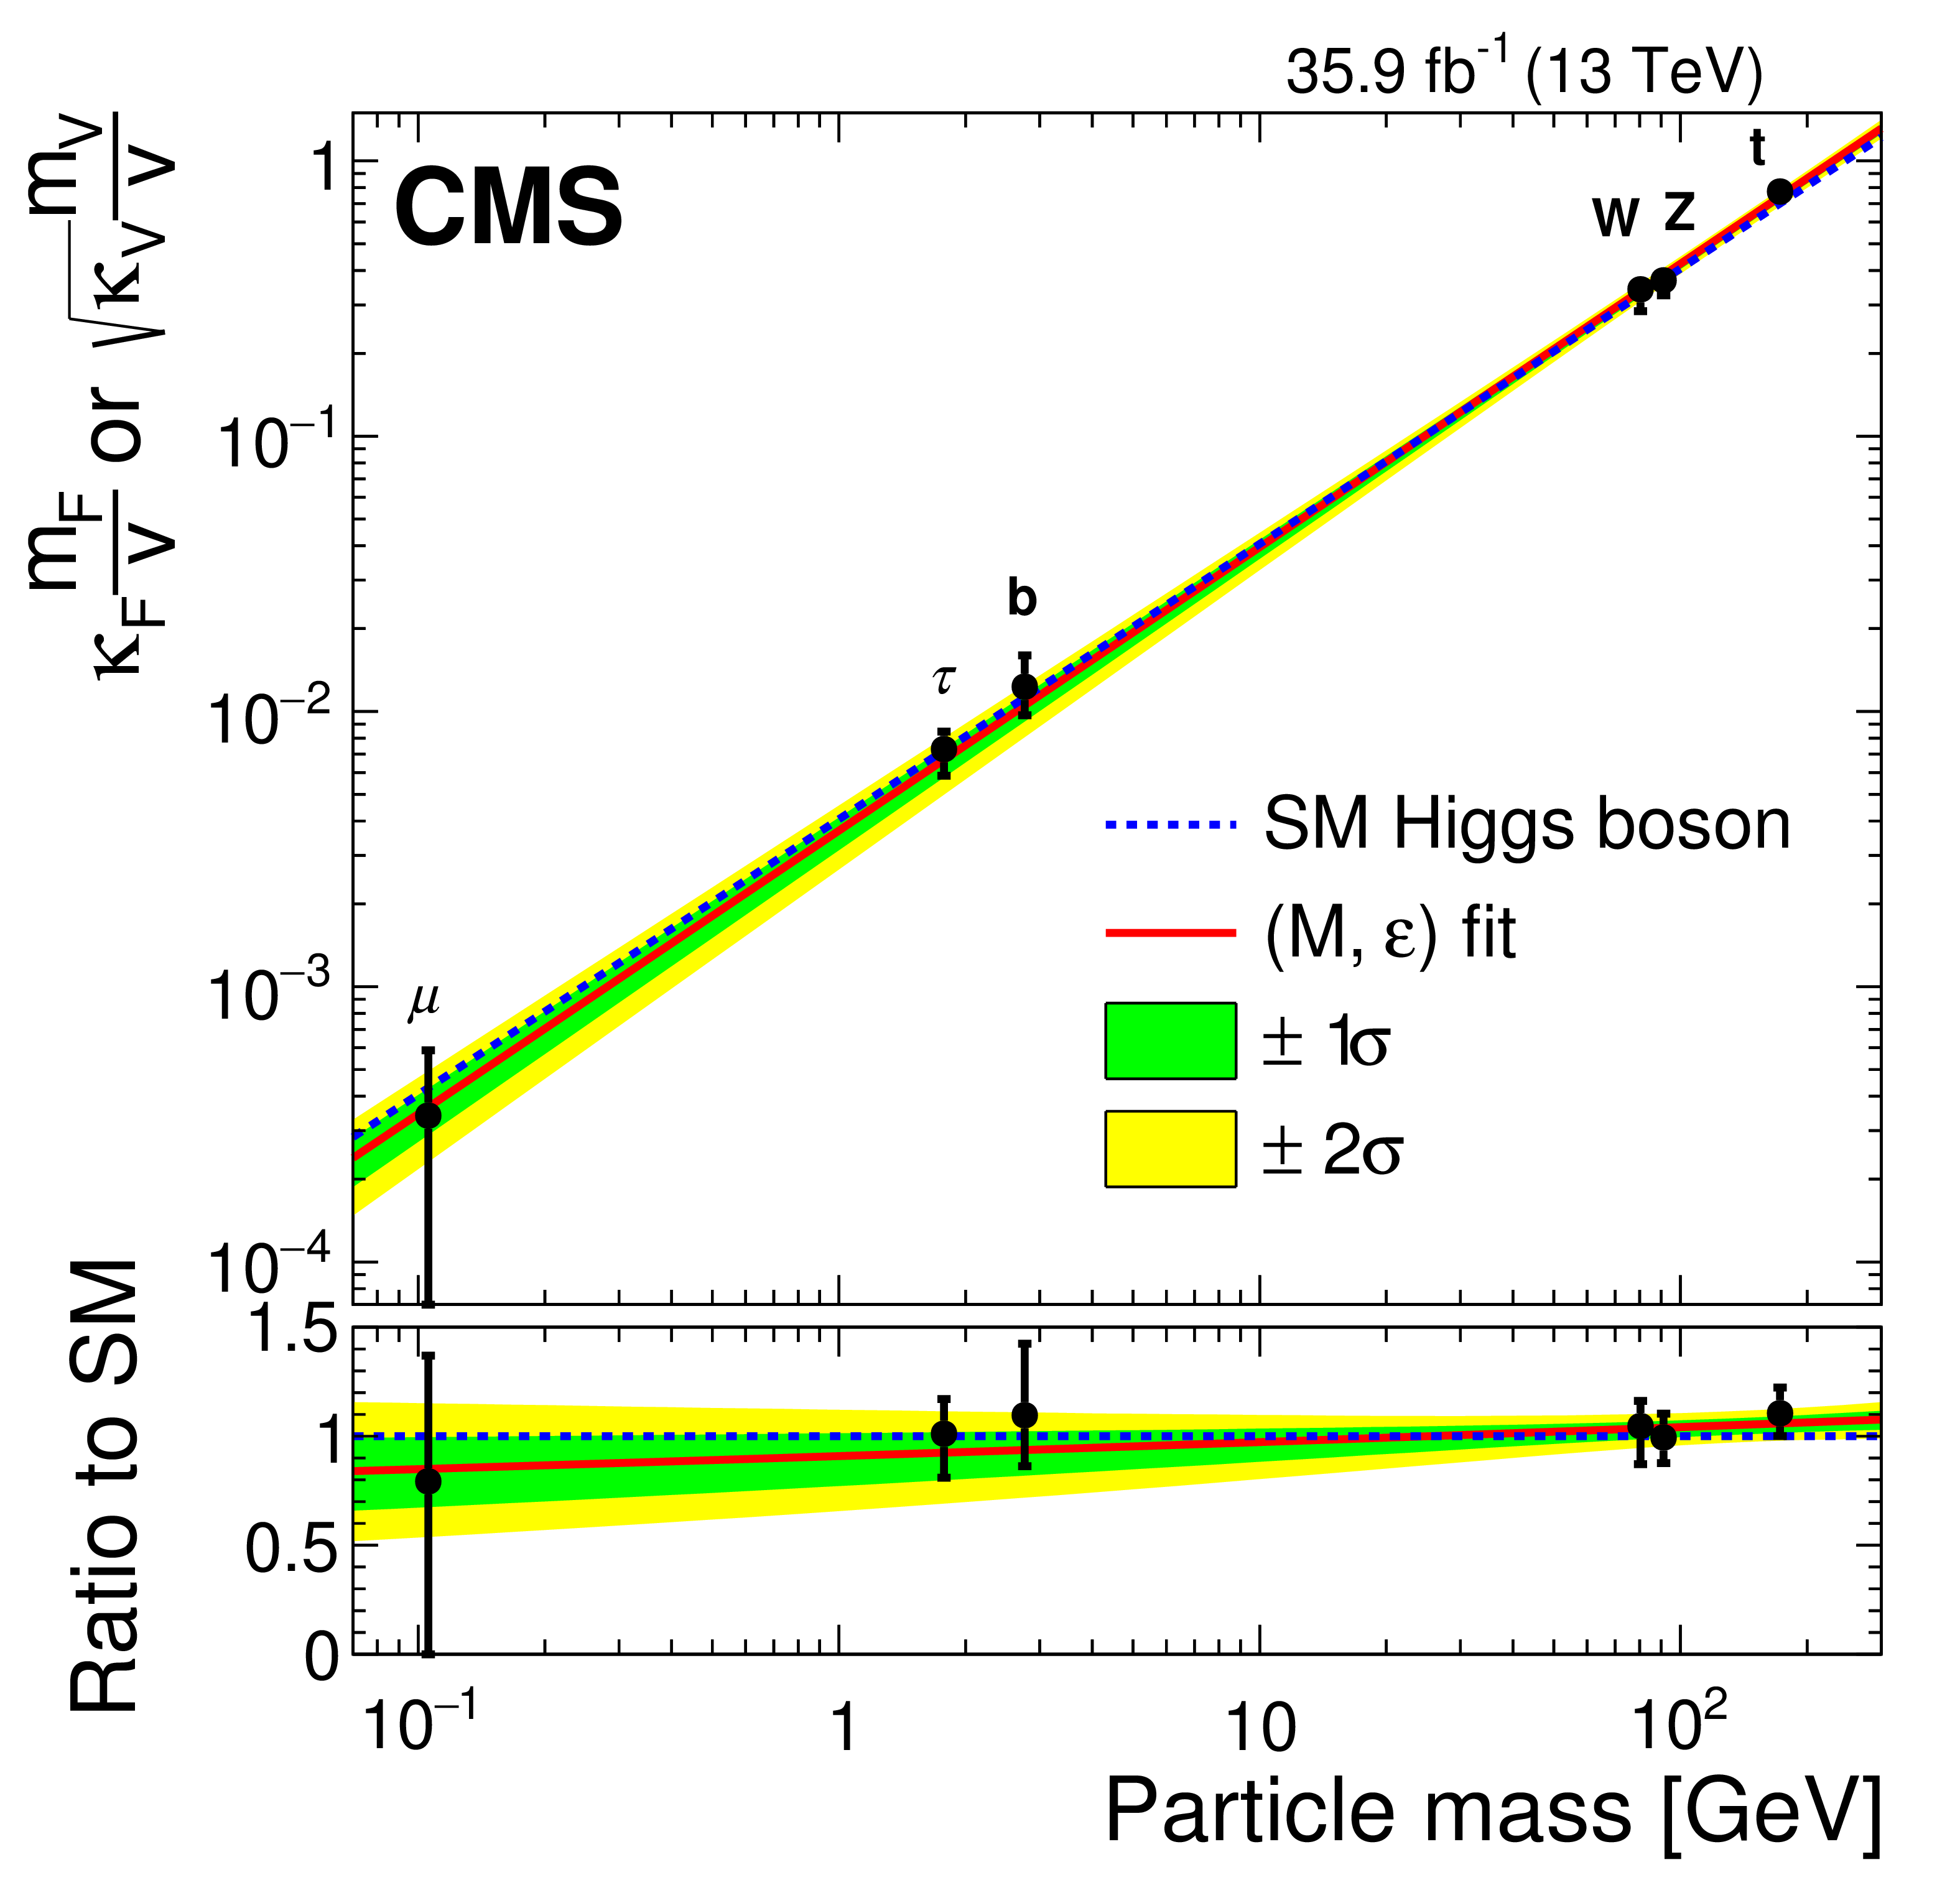
\includegraphics[width=0.60\textwidth]{pics/Intro/higgs_coupling_2016.png}
    \caption{Summary of the CMS measurements on the Higgs coupling to fermions and bosons.
             Plot taken from~\cite{Sirunyan:2640611}. }
    \label{fig:higgs_2016}
\end{figure*}



%\section{Potential anomaly coupling of Higgs to muons}